\documentclass[12pt]{article}
\usepackage{hyperref}
\usepackage[francais]{babel}
\usepackage[utf8]{inputenc}  
\usepackage[T1]{fontenc}
\usepackage{graphicx}

\title{\textbf{Projet Bases de Données :\\site de préférences vidéos}}
\author{Cyril Meyer\\
		cyril@adem.u-strasbg.fr\\
		Rapport de Modélisation}
\begin{document}

\date{}
\maketitle
\newpage

Notes pour le lecteur, les images du documents sont disponibles dans le dossier "annexes" fournis dans le dossier de rendu.

\section{Technologies utilisés}
Le projet à été crée en utilisant les technologies suivantes :\\

\begin{itemize}
\item Serveur Ubuntu 16.04.1 LTS
\item SGBD Oracle XE 10.2
\item Conception MCD/MLD JMerise
\item Environnement de développement Oracle SQL Developer
\end{itemize}

\section{Description du modèle}

\subsection{Table Users}
La table Users contient la liste des utilisateurs et leurs informations.
\subsubsection{Relations}
La tables est en relation avec les tables suivantes :
\begin{itemize}
\item Categories (via la table de relation Interested)
\item Emissions (via la table de relation Subscribe)
\item Episodes (via la table de relation Favorite)
\item History (via la relation HistoryRA)
\item Groups (via la table de relation BelongsTo)
\end{itemize}

\subsection{Table Categories}
La table Categories contient la liste des catégories d'émission.
\subsubsection{Relations}
La tables est en relation avec les tables suivantes :
\begin{itemize}
\item Users (via la table de relation Interested)
\item Emissions (via la relation TypeOfEmission)
\end{itemize}

\subsection{Table Emissions}
La table Emissions contient la liste des émissions existantes.
\subsubsection{Relations}
La tables est en relation avec les tables suivantes :
\begin{itemize}
\item Episodes (via la relation Contain)
\item Archives (via la relation ContainArchive)
\item Categories (via la relation TypeOfEmission)
\end{itemize}

\subsection{Table Groups}
La table Groups contient la liste des groupes de droits (administration).
\subsubsection{Relations}
La tables est en relation avec la tables suivante :
\begin{itemize}
\item Users (via la table de relation BelongsTo)
\end{itemize}

\subsection{Table History}
La table History contient la liste des visionnages d'épisodes.
\subsubsection{Relations}
La tables est en relation avec les tables suivantes :
\begin{itemize}
\item Users (via la relation HistoryRA)
\item Episodes (via la relation HistoryRB)
\end{itemize}

\subsection{Table Episodes}
La table Episodes contient la liste des épisodes d'émissions disponible au visionnage.
\subsubsection{Relations}
La tables est en relation avec les tables suivantes :
\begin{itemize}
\item Users (via la table de relation Favorite)
\item Emissions (via la relation Contain)
\item History (via la relation HistoryRB)
\end{itemize}

\subsection{Table Archives}
La table Archives contient la liste des épisodes d'émissions non-disponible au visionnage.
\subsubsection{Relations}
La tables est en relation avec les tables suivantes :
\begin{itemize}
\item Emissions (via la relation ContainArchive)
\end{itemize}

\section{Modèle conceptuel des données}
\vspace{5mm}
\center
\makebox[\textwidth]{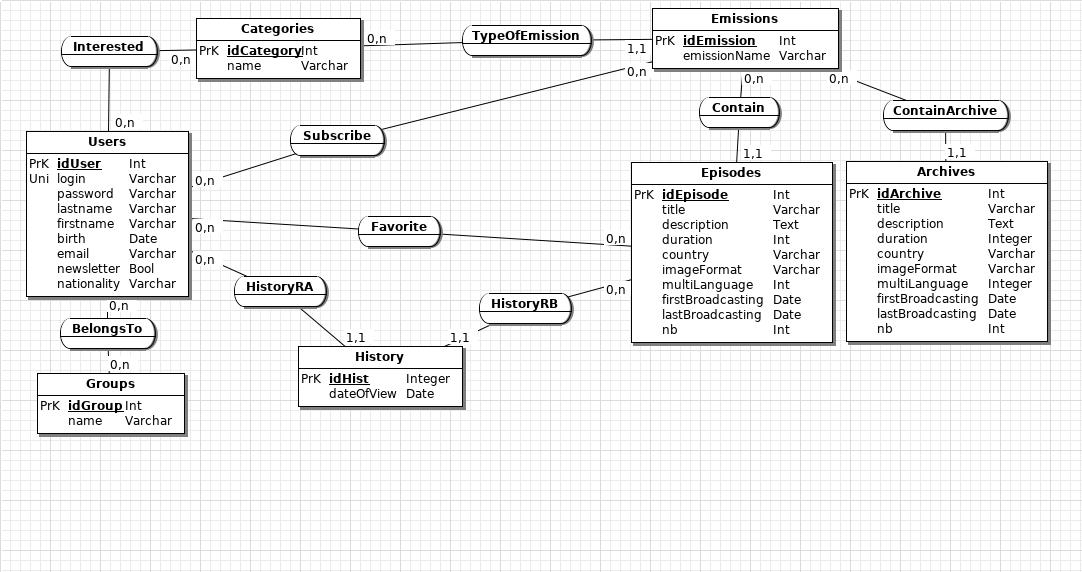
\includegraphics[width=200mm]{./annexes/mcd.jpg}}

\section{Modèle logique des données}
\vspace{5mm}
\center
\makebox[\textwidth]{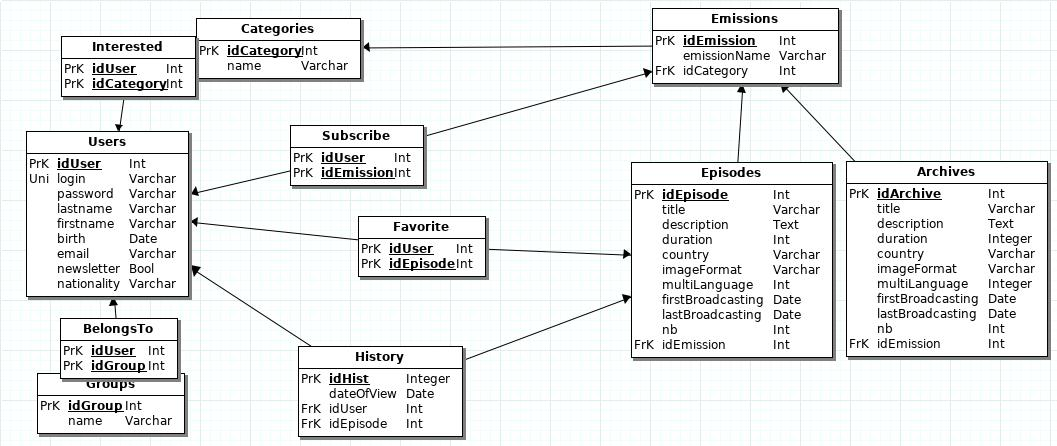
\includegraphics[width=200mm]{./annexes/mld.jpg}}

\section{Description du rendu}
Le rendu du projet est composé des fichiers suivants :
\begin{itemize}
\item RapportModelisation.pdf : Rapport de la modélisation du projet
\item annexes/mcd.jpg : MCD au format jpeg
\item annexes/mld.jpg : MLD au format jpeg
\item drop\_create.sql : script de création, suppression des tables
\item insert.sql : script d'insertion de données de tests
\item select.sql : script des requêtes SQL demandés
\item plsql.sql : script des Procédures et fonctions PL/SQL demandés
\item trigger.sql : script des Contraintes d’intégrité
\end{itemize}


\end{document}